\chapter{Workload Surveys} \label{appendix:workload}

\begin{figure}[tbp]
    \begin{center}
        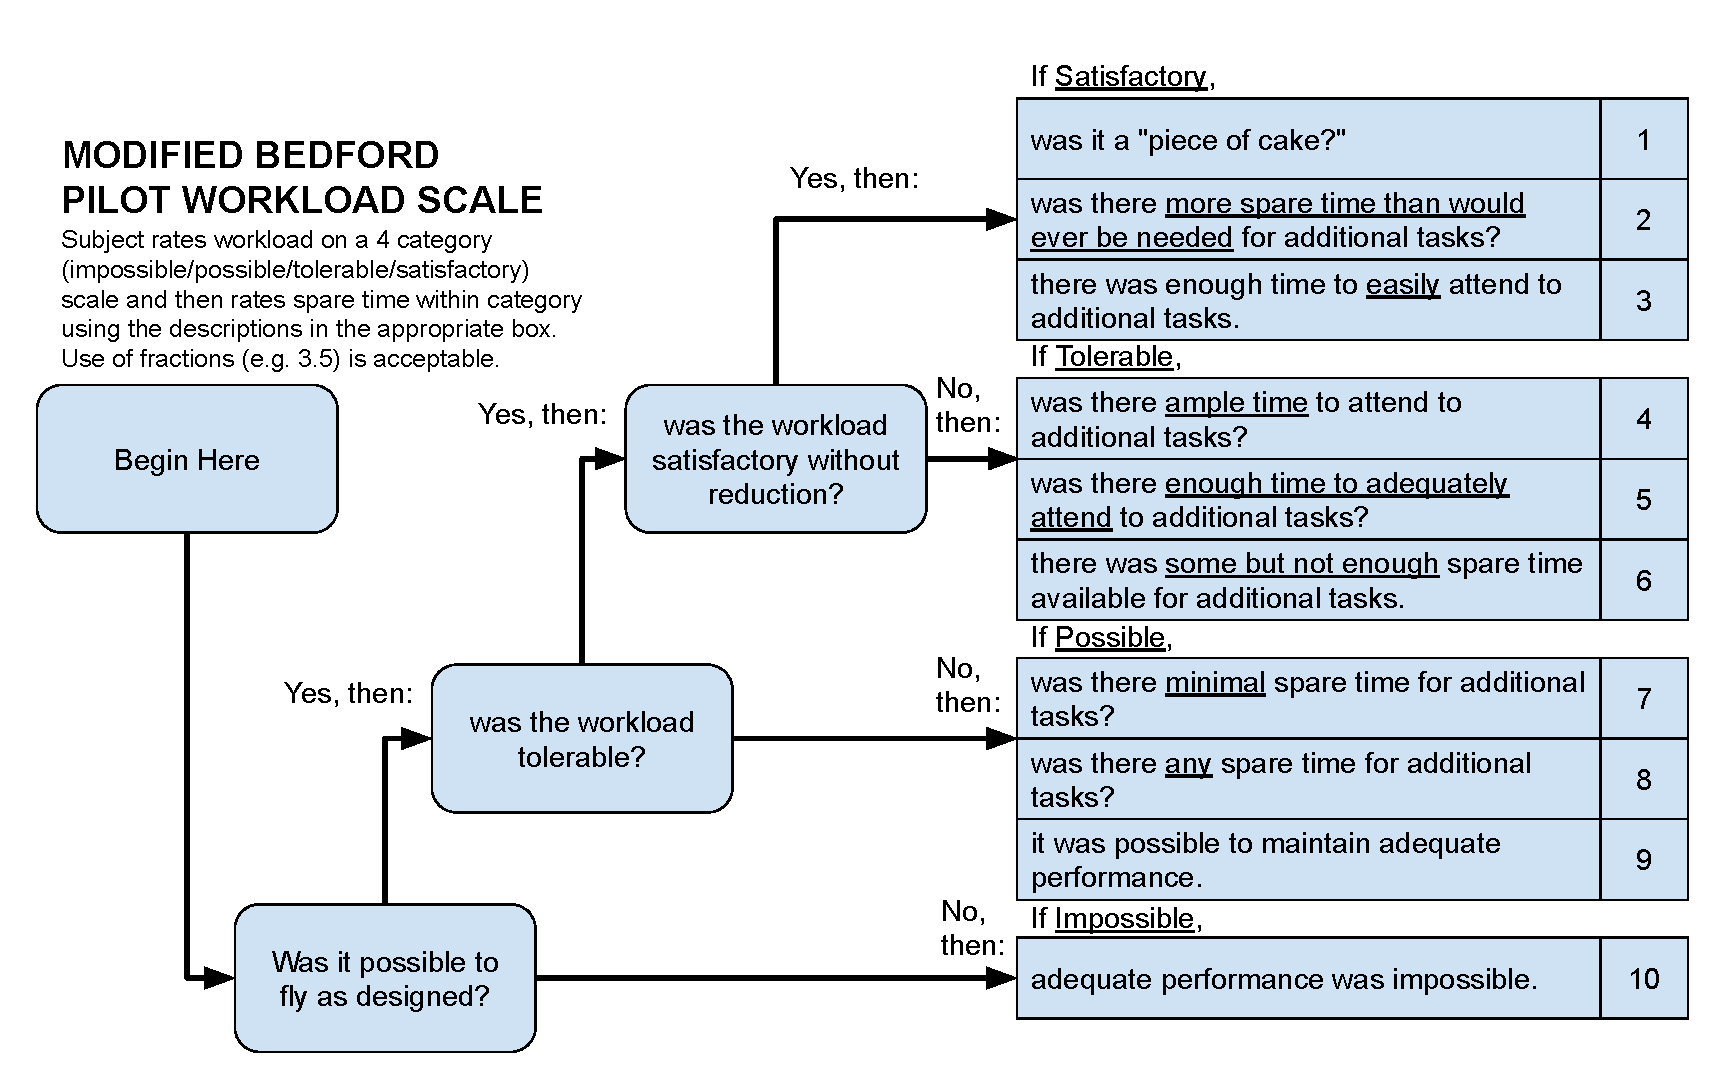
\includegraphics[width=1.4\linewidth,angle=90]{figures/Introduction/MODIFIED_BEDFORD_PILOT_WORKLOAD_SCALE.pdf}
        \caption[The Modified Bedford Workload Scale]{The Modified Bedford Workload Scale, adapted from~\citet{roscoe_subjective_1990}.}
        \label{figure:modifiedbedford}
    \end{center}
\end{figure}

% \begin{figure}[ht]
%     \begin{adjustbox}{addcode={\begin{minipage}{\width}}{\caption[The Modified Bedford Workload Scale]{The Modified Bedford Workload Scale, adapted from~\citet{roscoe_subjective_1990}.}\end{minipage}},rotate=90,center}
%         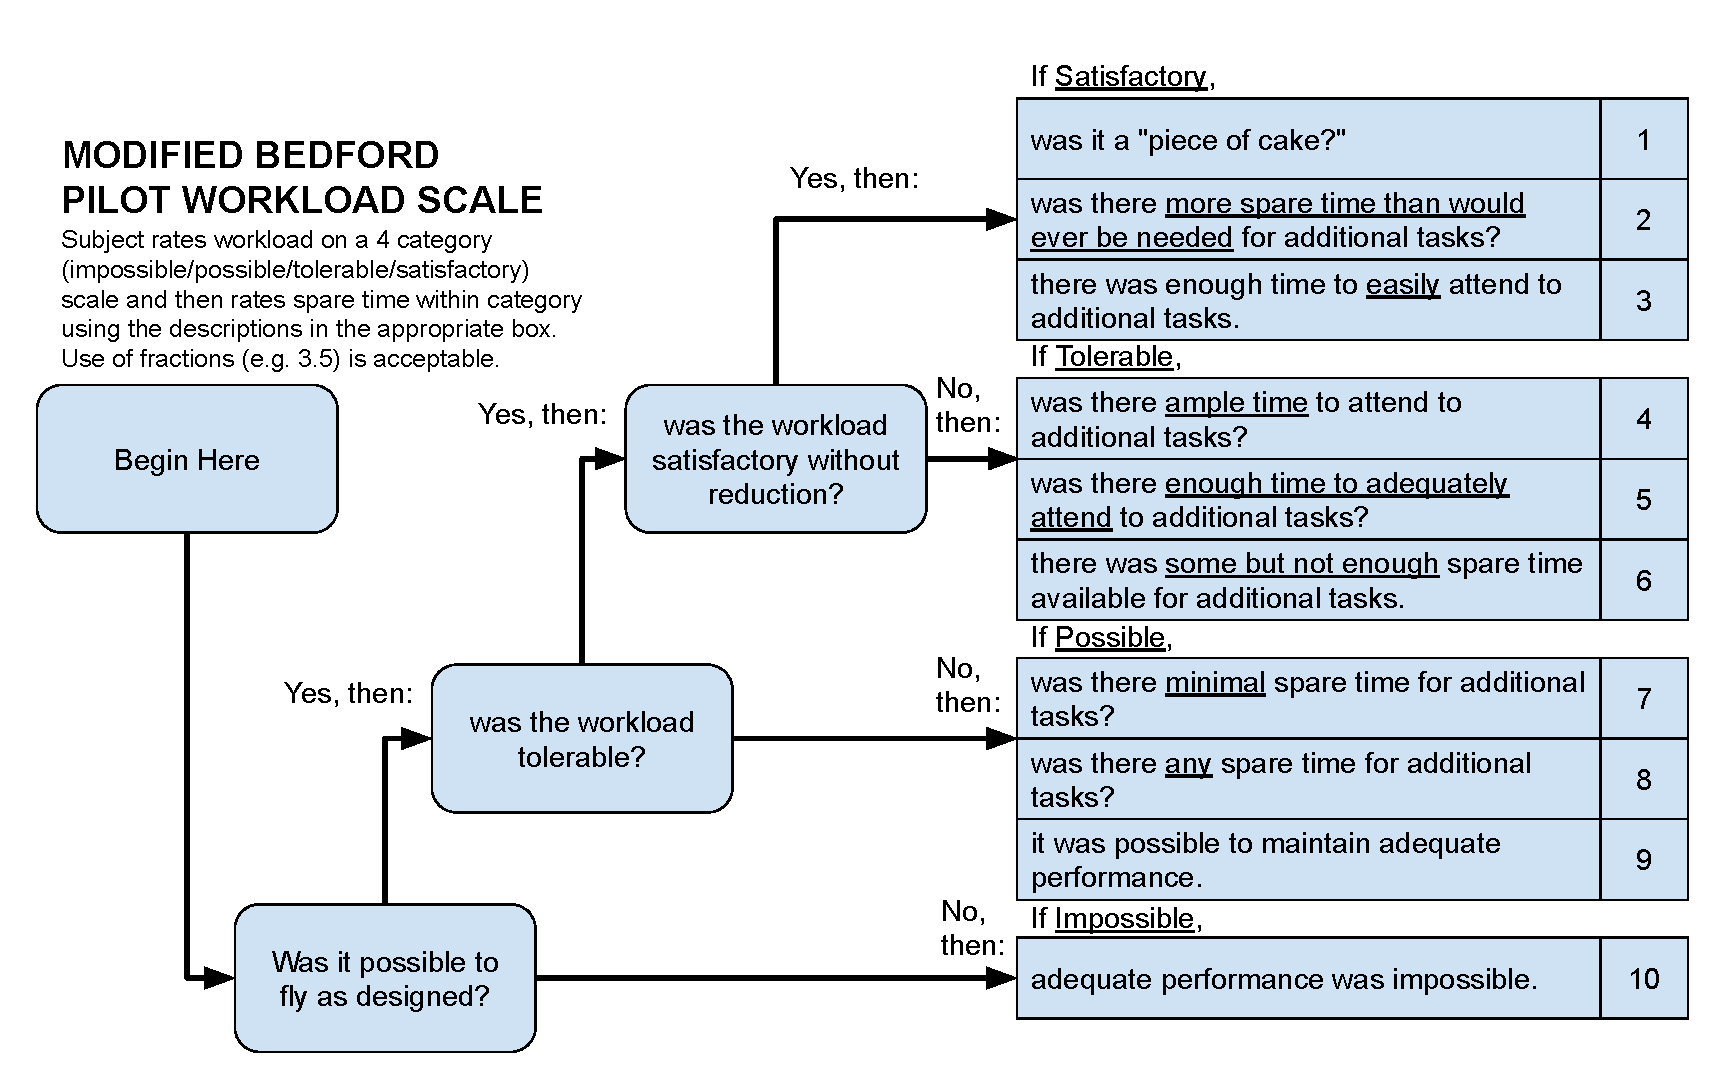
\includegraphics[width=1.4\linewidth]{figures/Introduction/MODIFIED_BEDFORD_PILOT_WORKLOAD_SCALE.pdf}%
%         \label{figure:modifiedbedford}
%     \end{adjustbox}
% \end{figure}

\begin{figure}[tbp]
    \begin{center}
        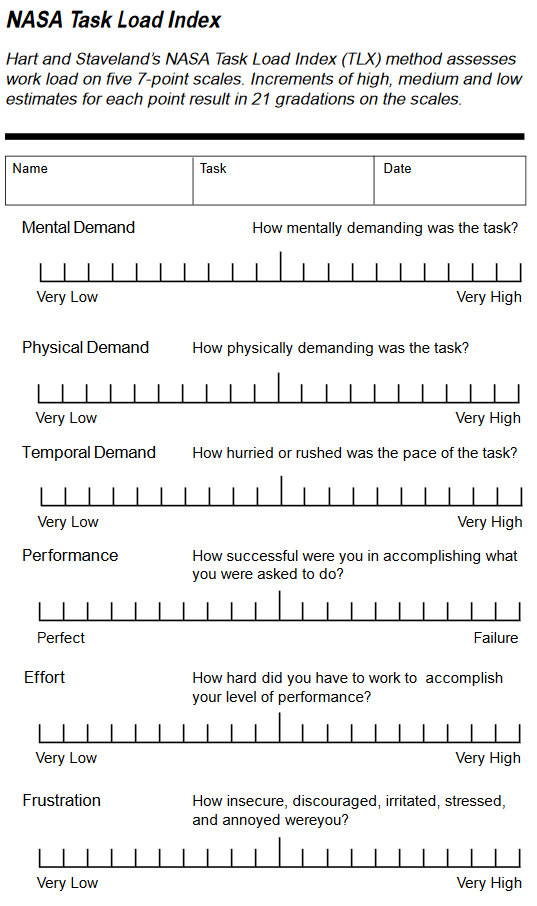
\includegraphics[width=0.8\linewidth]{figures/Introduction/NASA-TLX.png}
        \caption[The NASA Task Load Index (NASA-TLX)]{The NASA Task Load Index (NASA-TLX), from~\citet{hart_development_1988}.}
        \label{figure:nasa-tlx}
    \end{center}
\end{figure}

\chapter{Trade Analysis Tables} \label{appendix:trade-tables}

\begin{figure}[b!]
    \begin{center}
        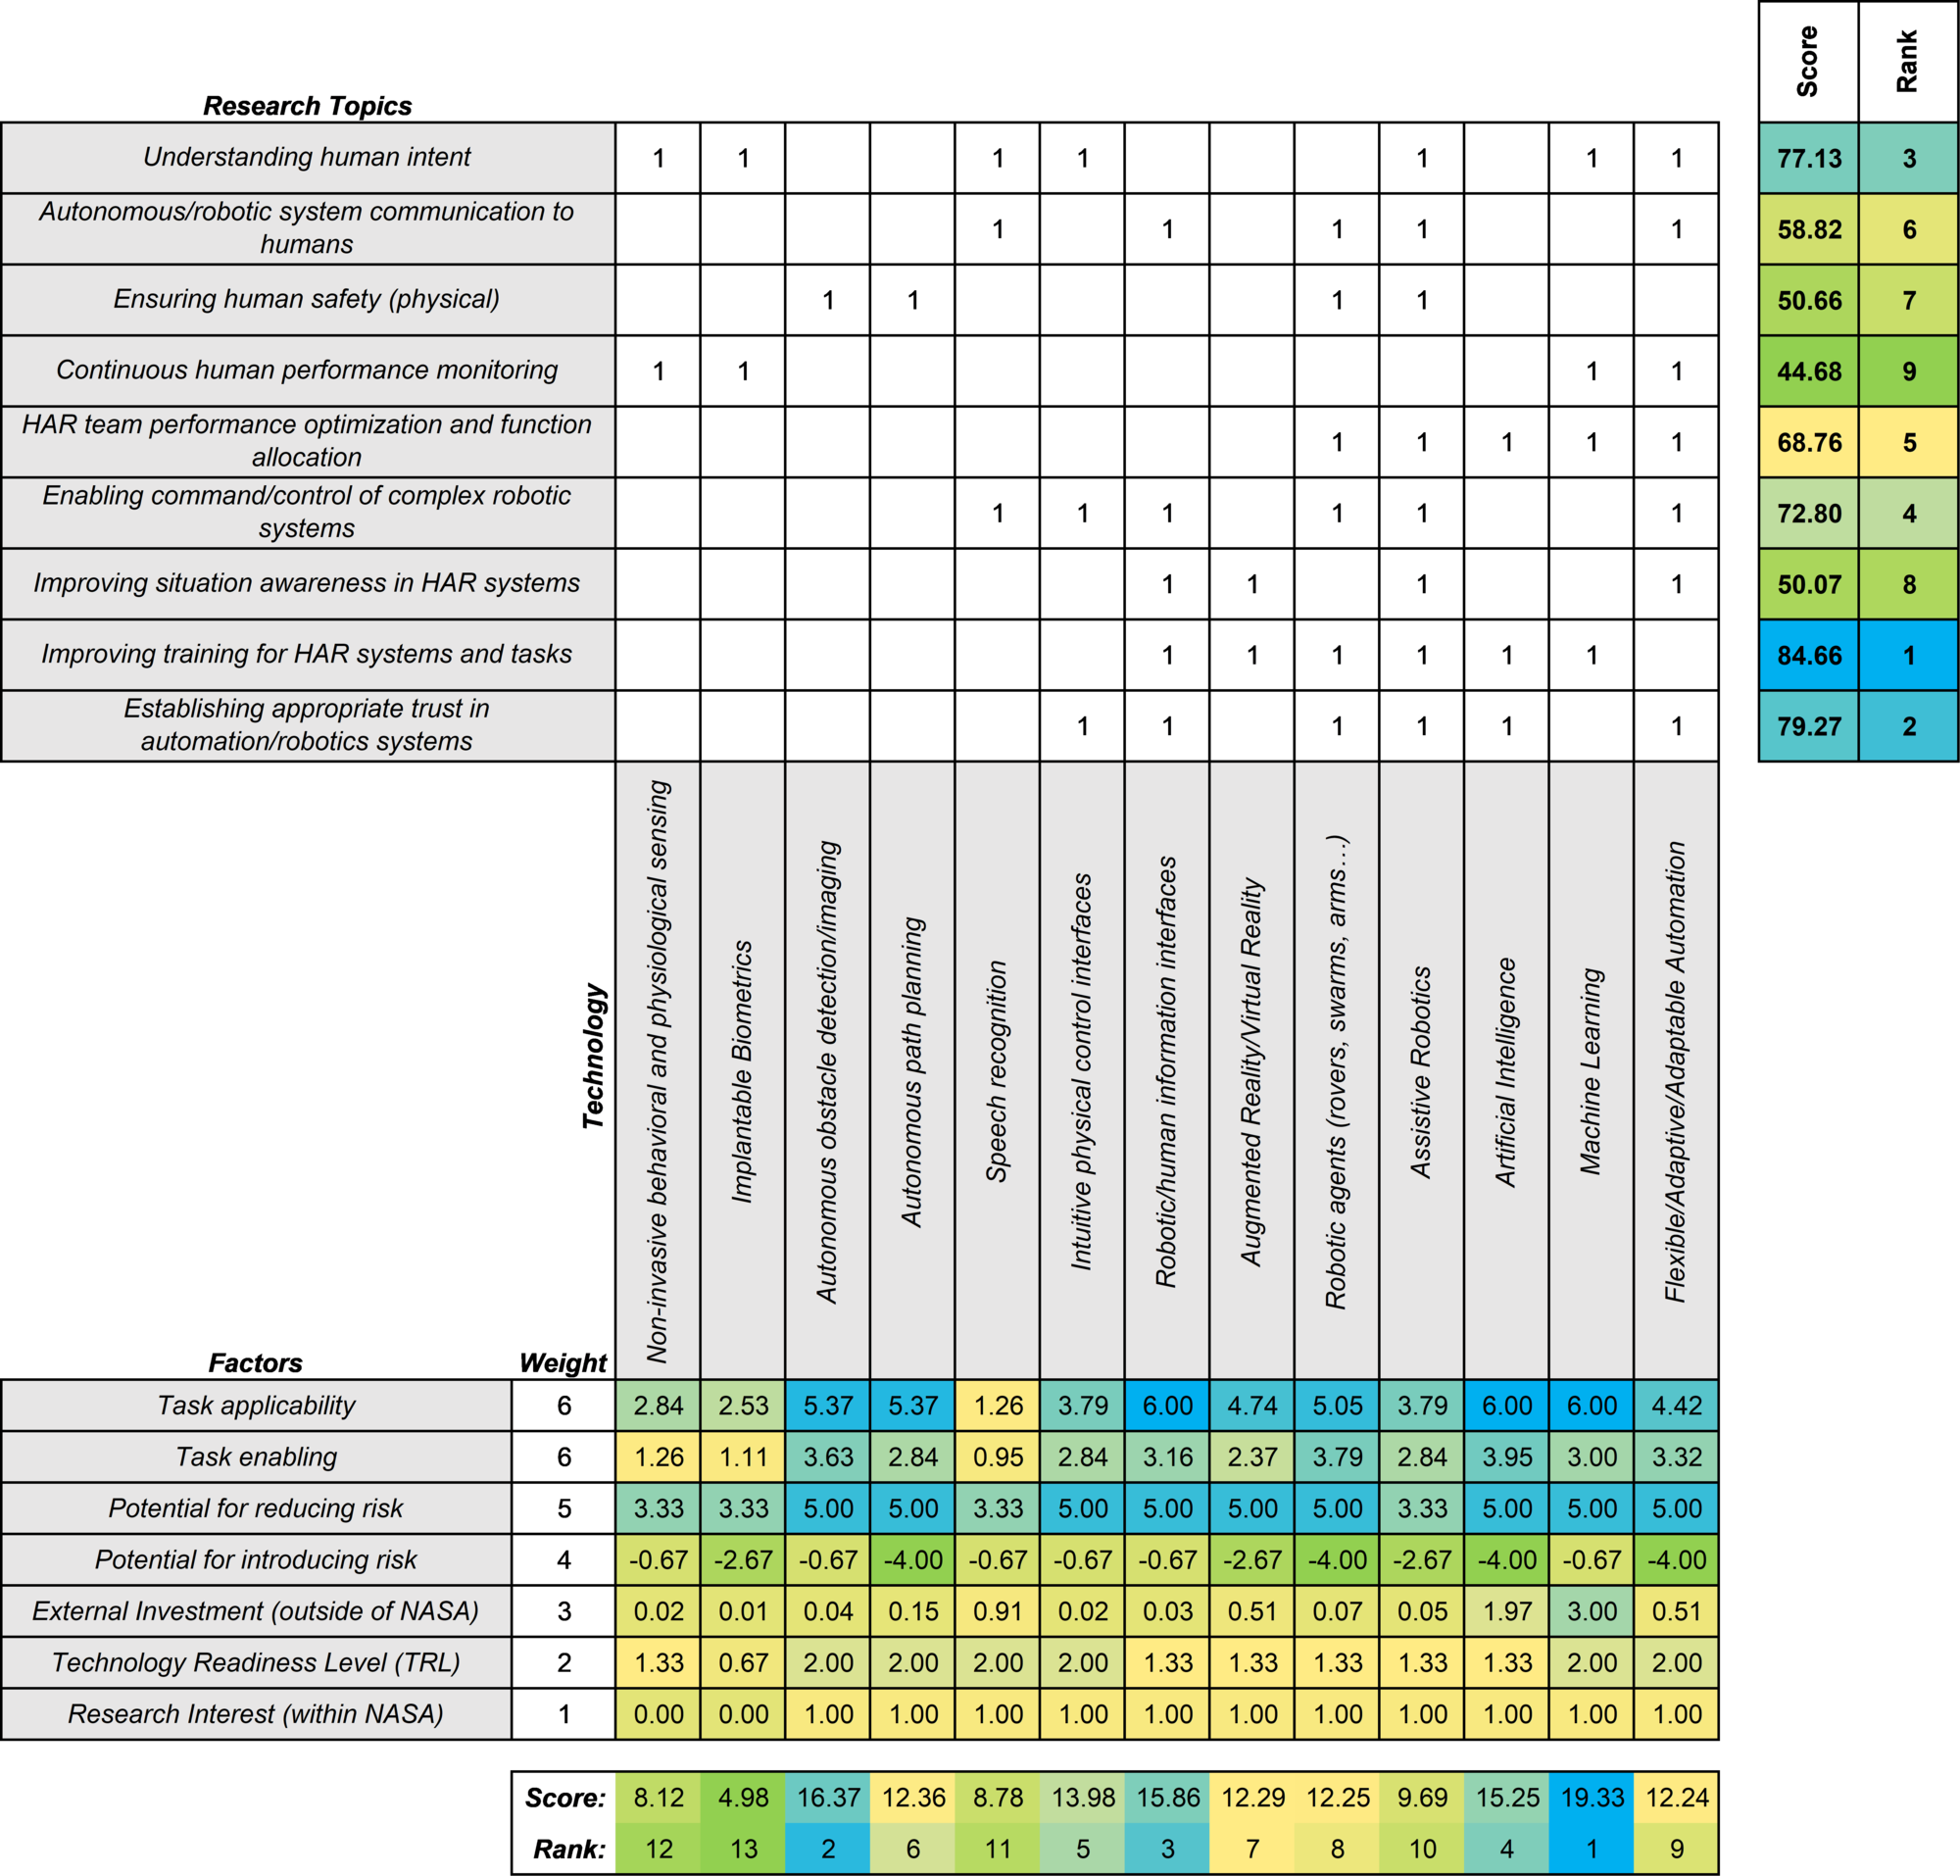
\includegraphics[width=0.8\linewidth]{figures/TradeStudy/figurea1.png}
        \caption[Top-level trade table]{Top-level trade table with final research topic scores (top right), final technology scores based on factors (bottom) and weighted factor-level scores for each technology.}
        % \label{figure:}
    \end{center}
\end{figure}

\begin{figure}[b!]
    \begin{center}
        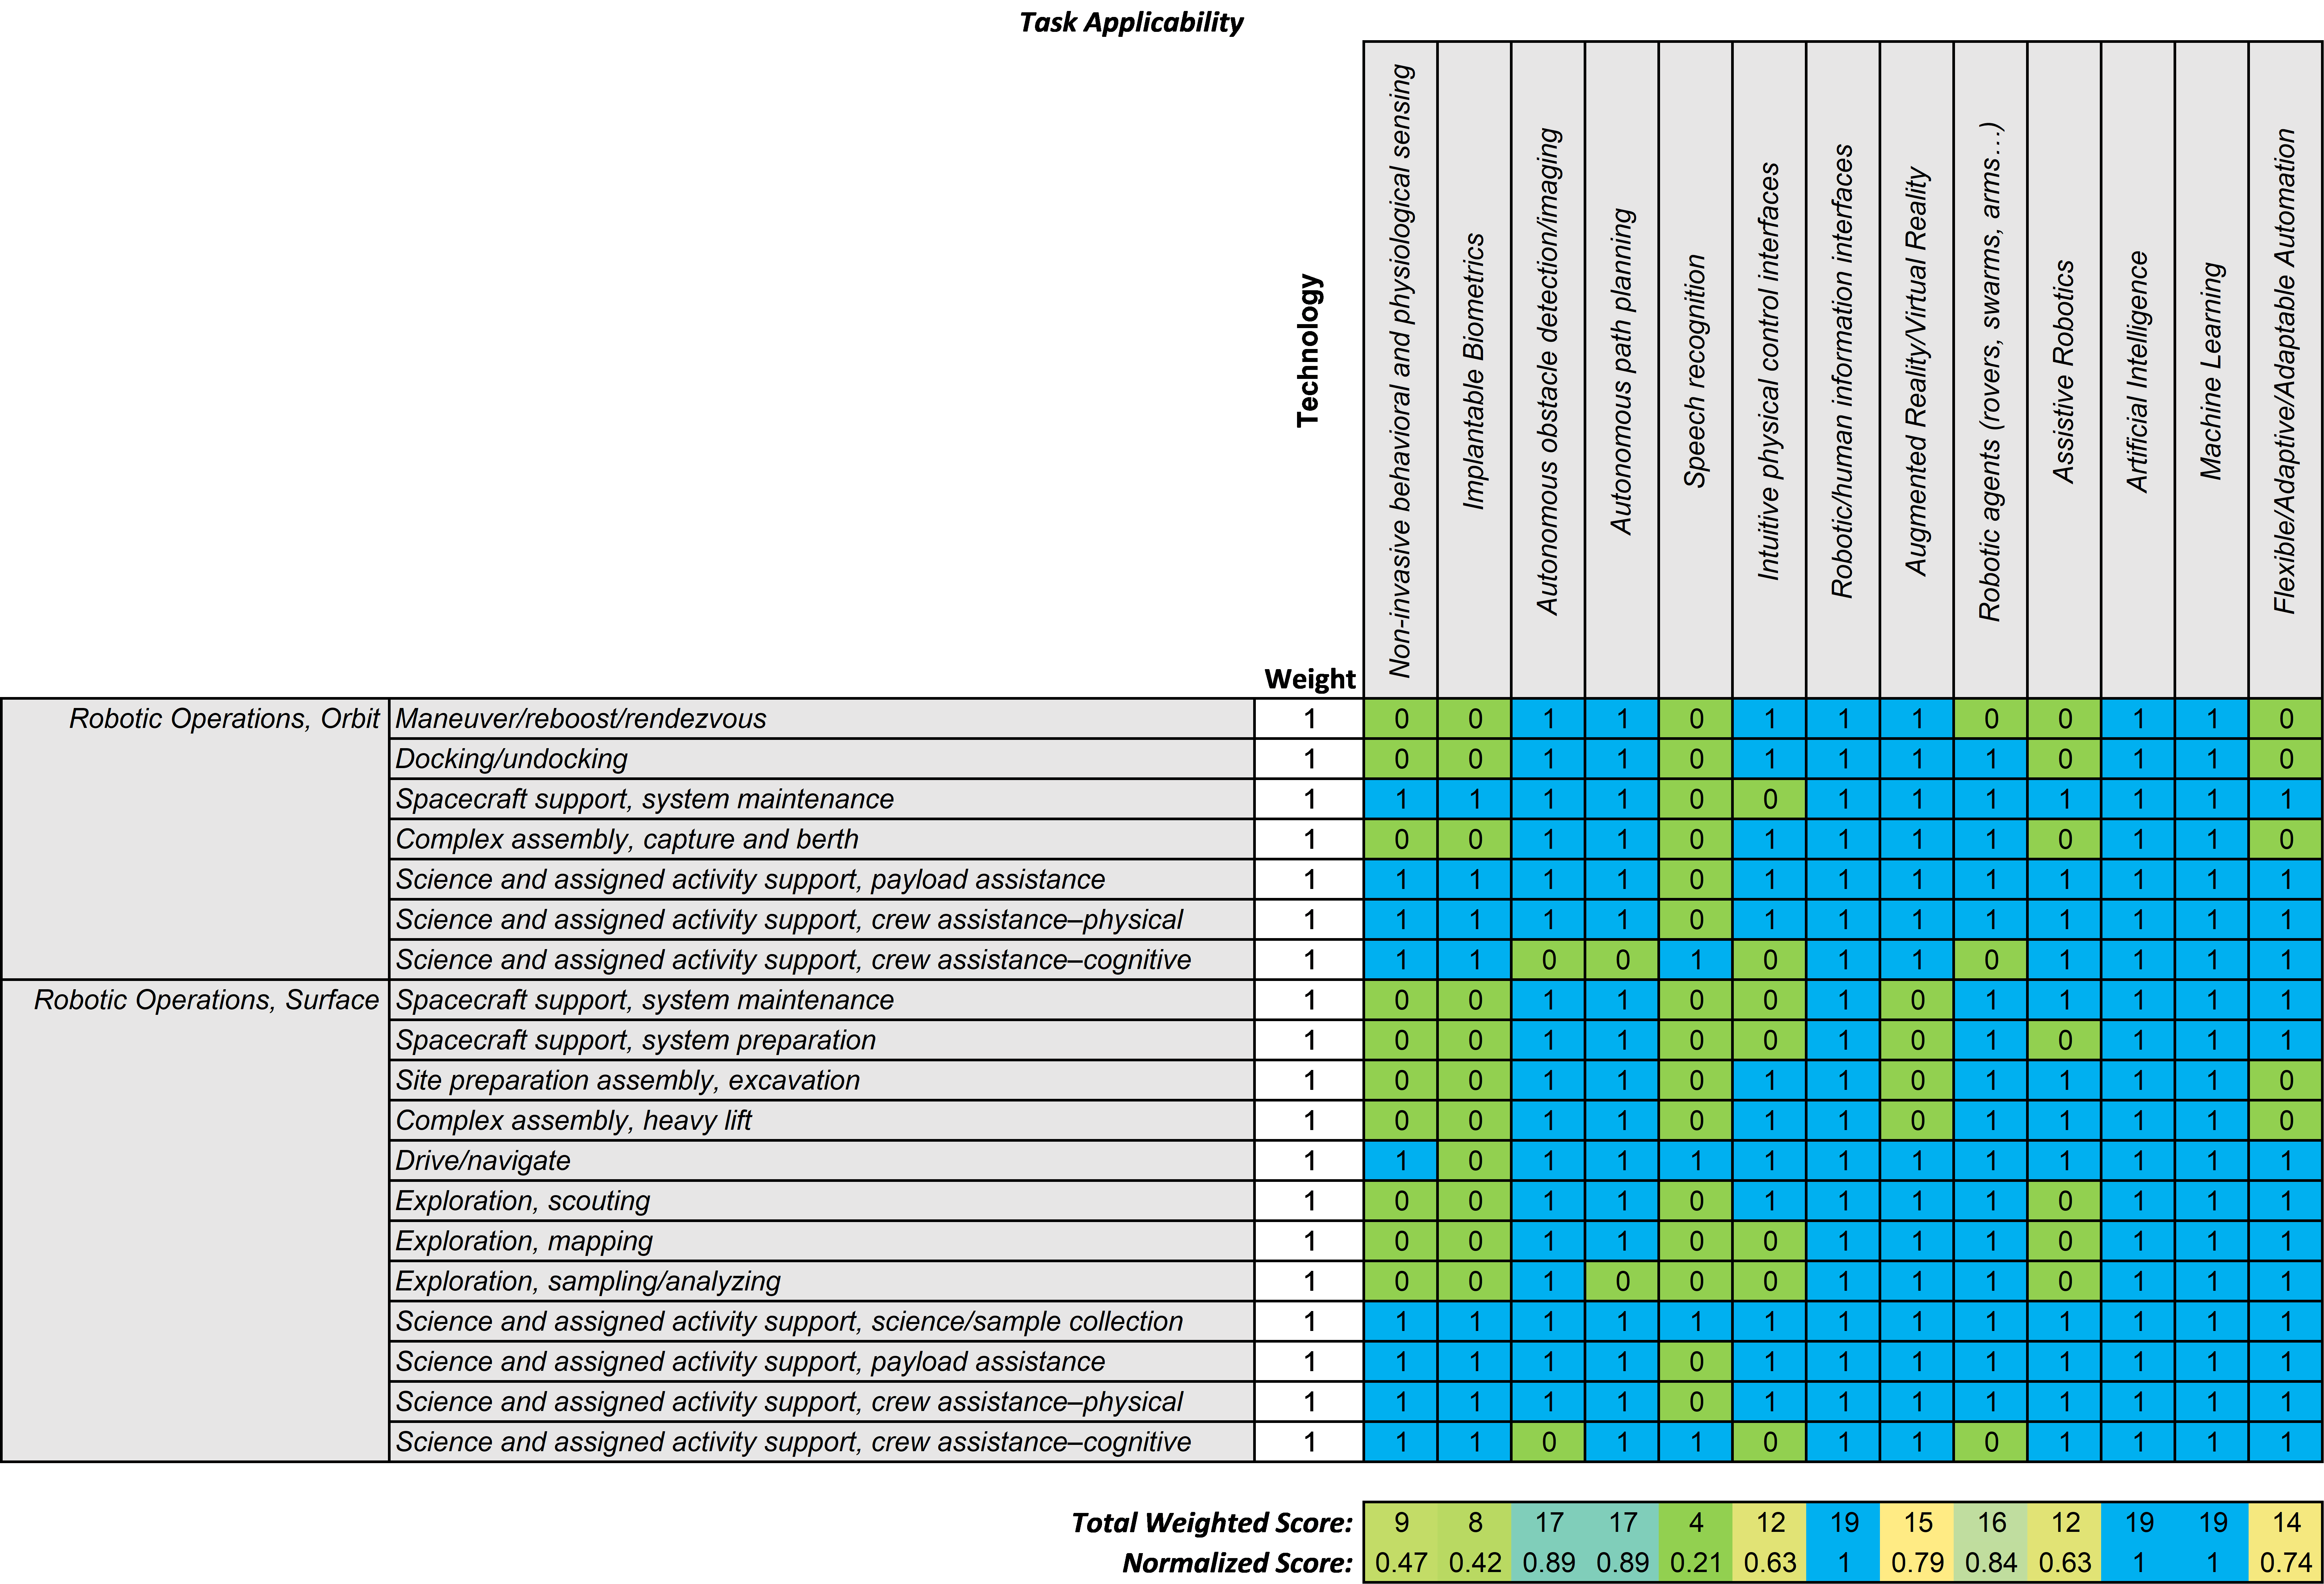
\includegraphics[width=0.8\linewidth]{figures/TradeStudy/figurea2.png}
        \caption[Technology to Task Applicability factor-level trade table]{Technology to Task Applicability factor-level trade table.}
        % \label{figure:}
    \end{center}
\end{figure}

\begin{figure}[b!]
    \begin{center}
        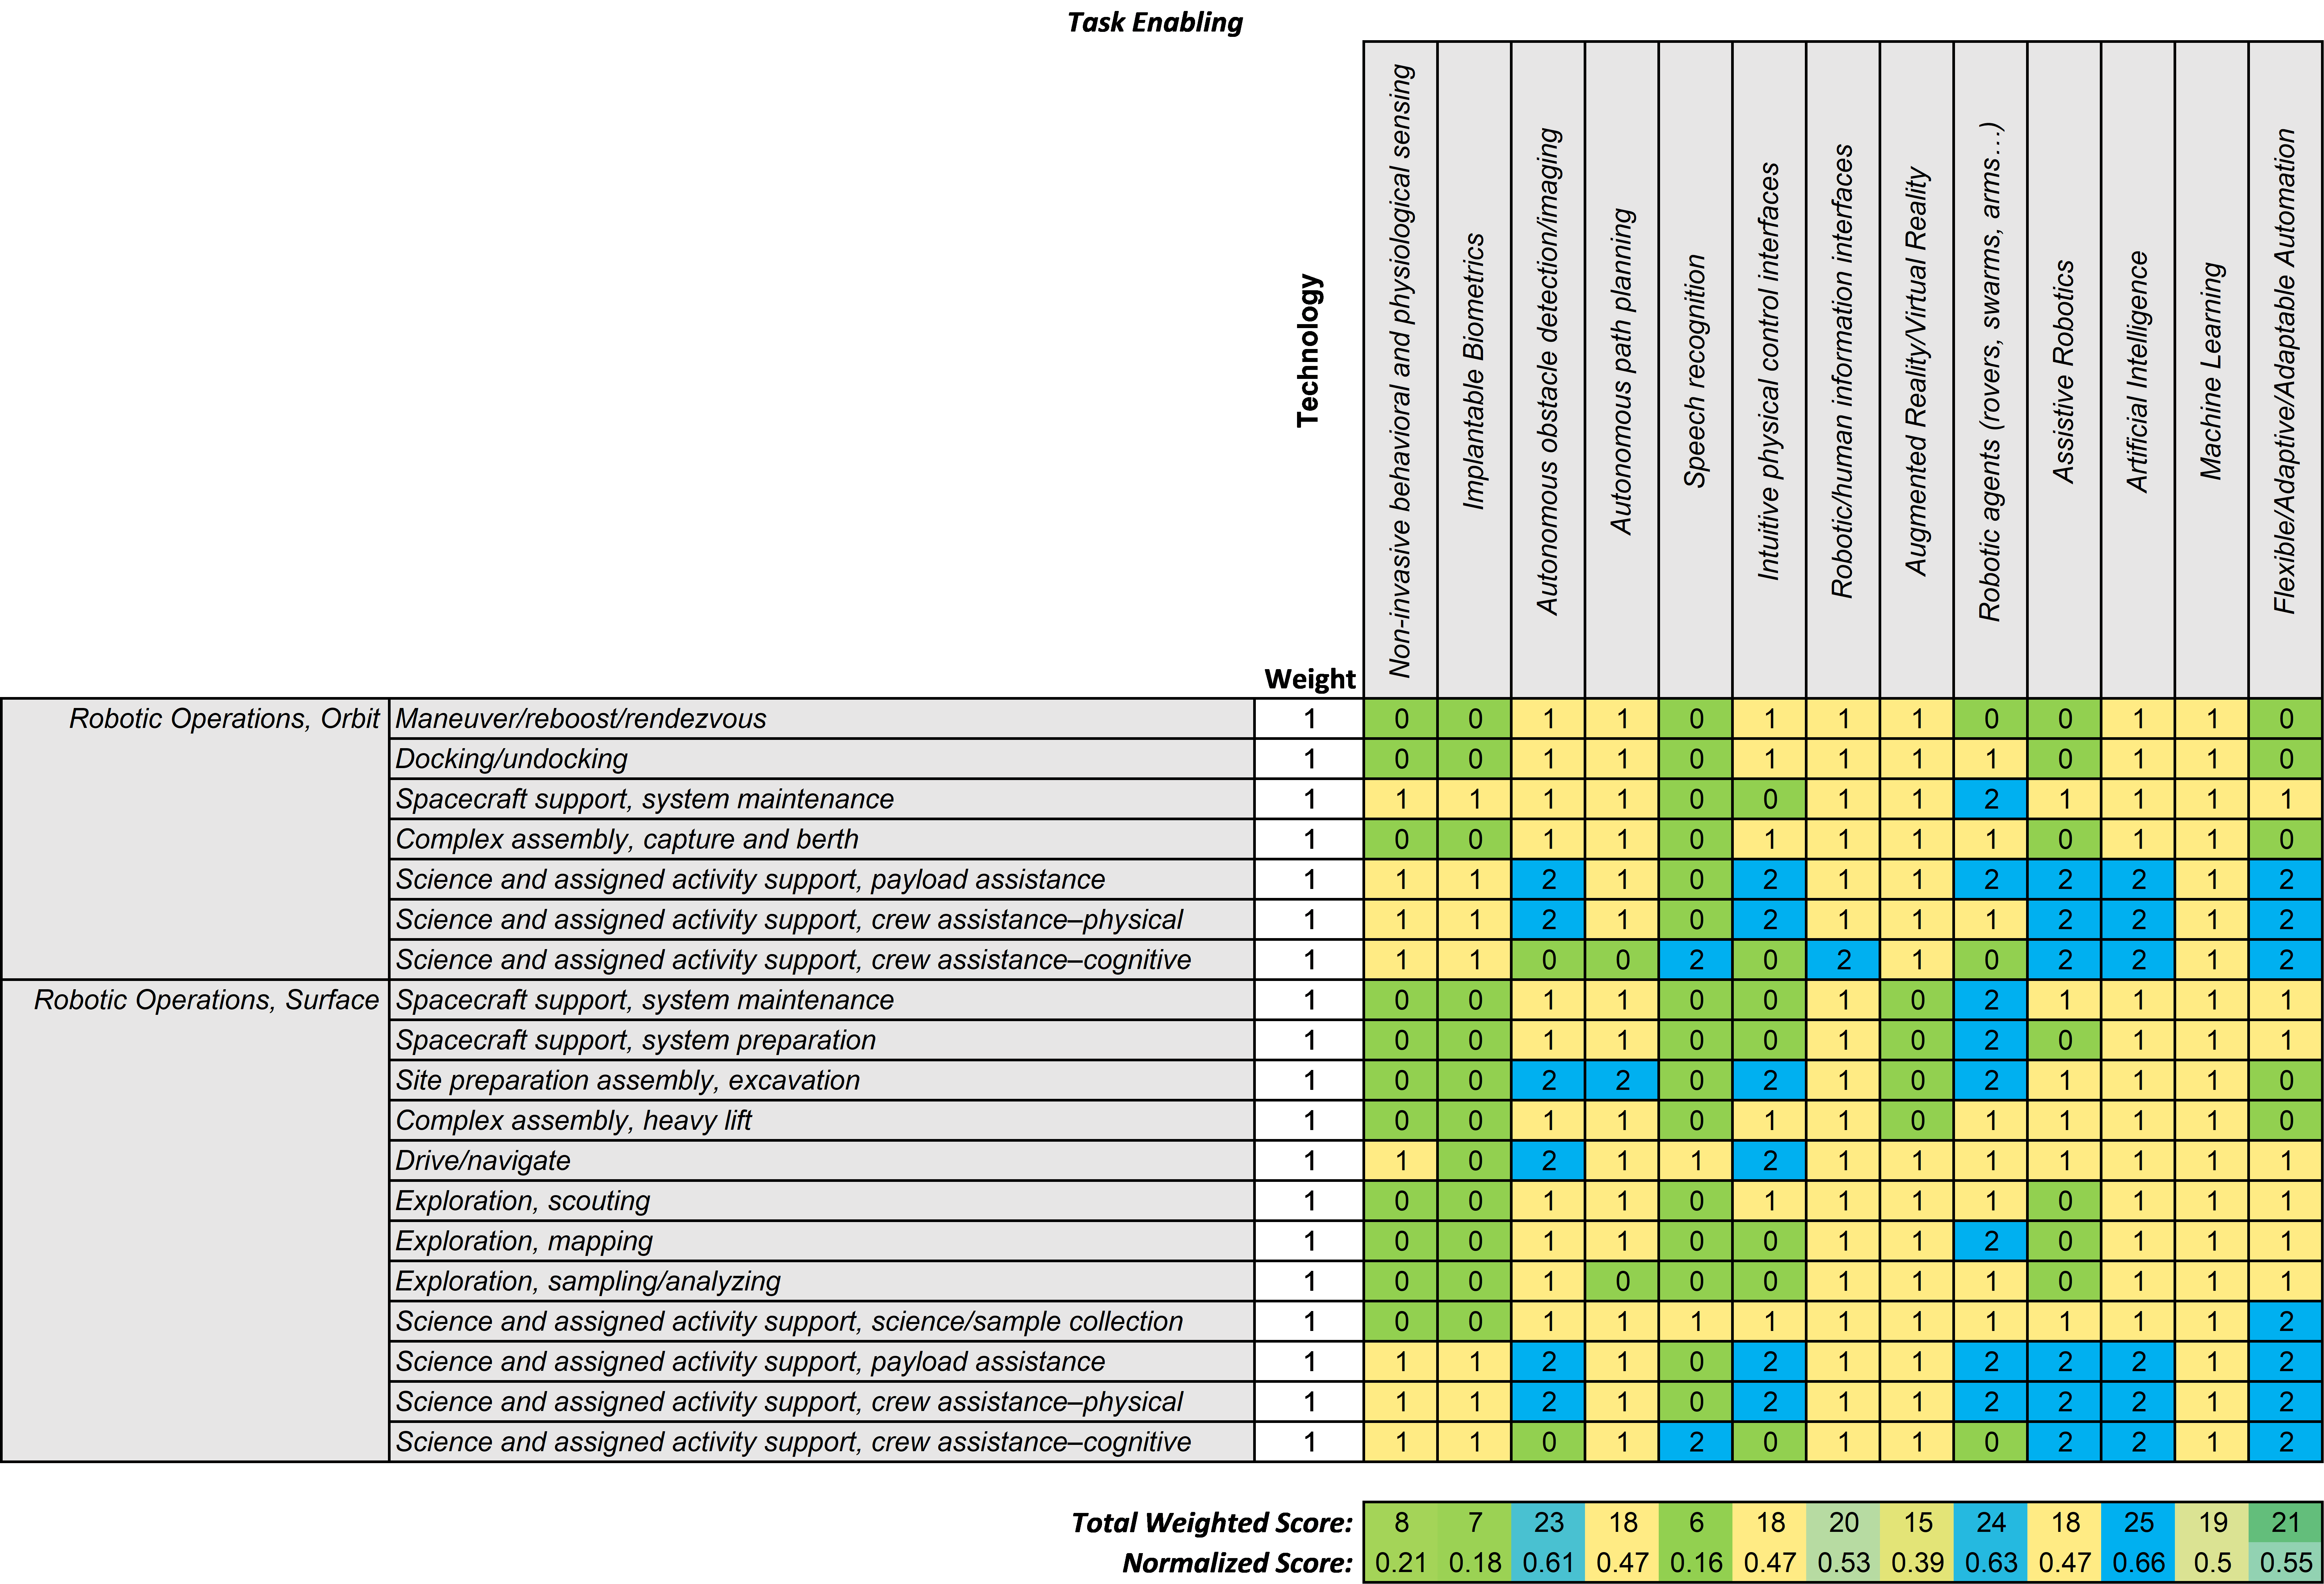
\includegraphics[width=0.8\linewidth]{figures/TradeStudy/figurea3.png}
        \caption[Technology to Task Enabling factor-level trade table]{Technology to Task Enabling factor-level trade table.}
        % \label{figure:}
    \end{center}
\end{figure}

\begin{figure}[b!]
    \begin{center}
        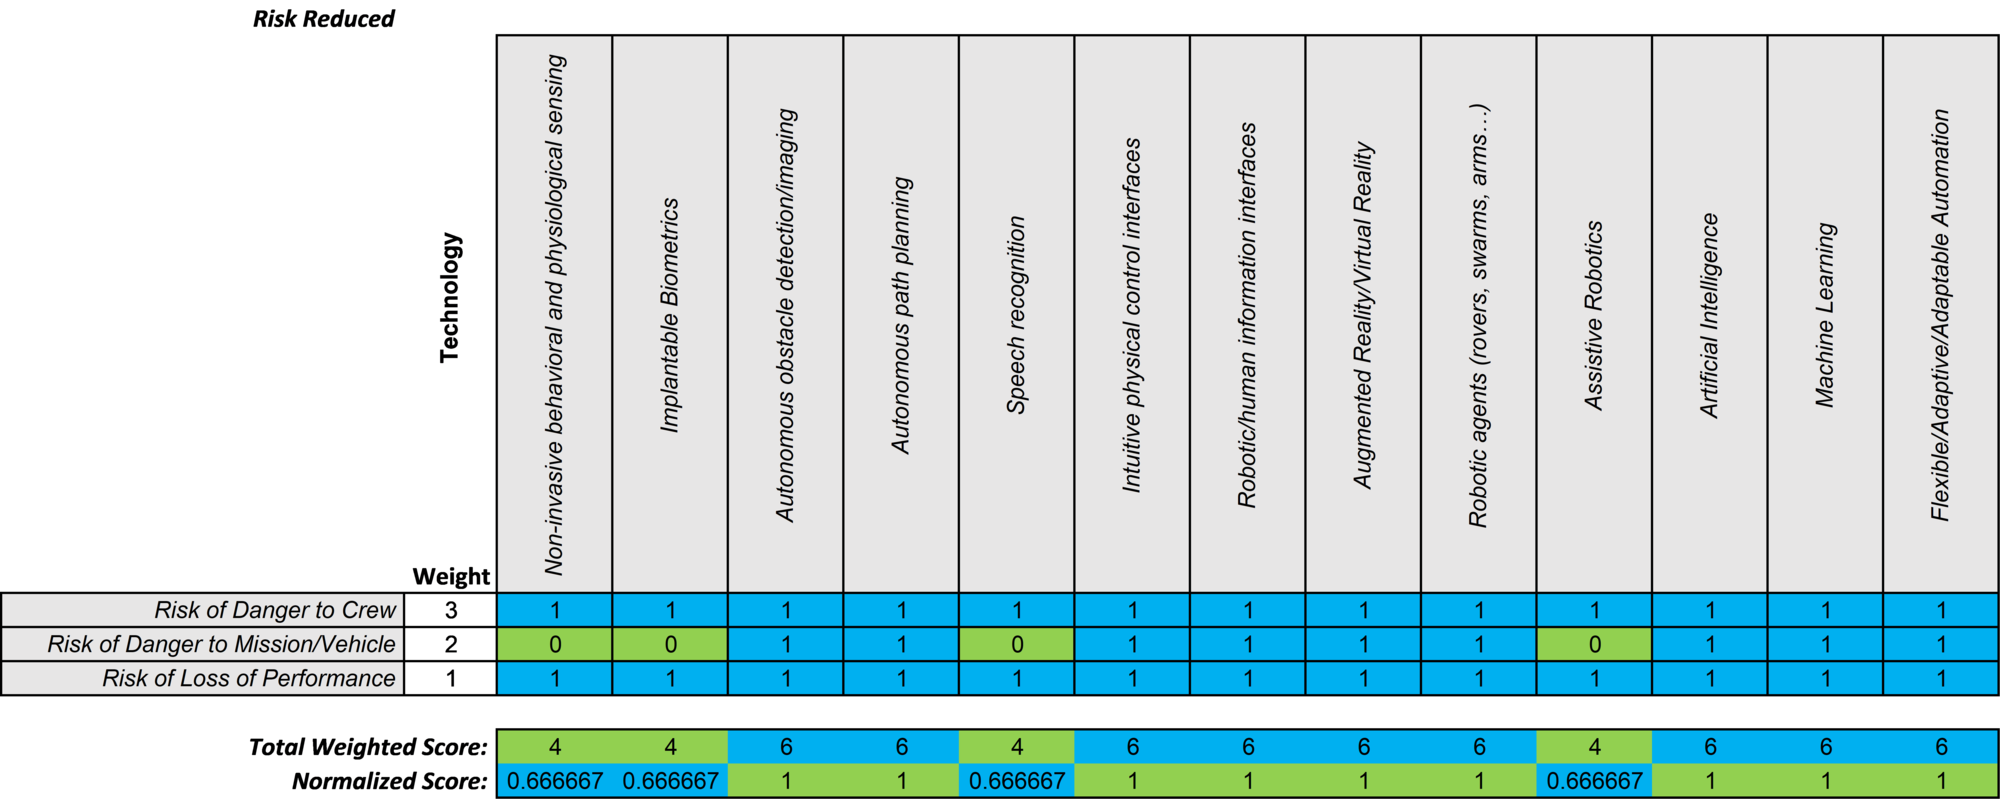
\includegraphics[width=0.8\linewidth]{figures/TradeStudy/figurea4.png}
        \caption[Technology to Risk Reduced factor-level trade table]{Technology to Risk Reduced factor-level trade table.}
        % \label{figure:}
    \end{center}
\end{figure}

\begin{figure}[b!]
    \begin{center}
        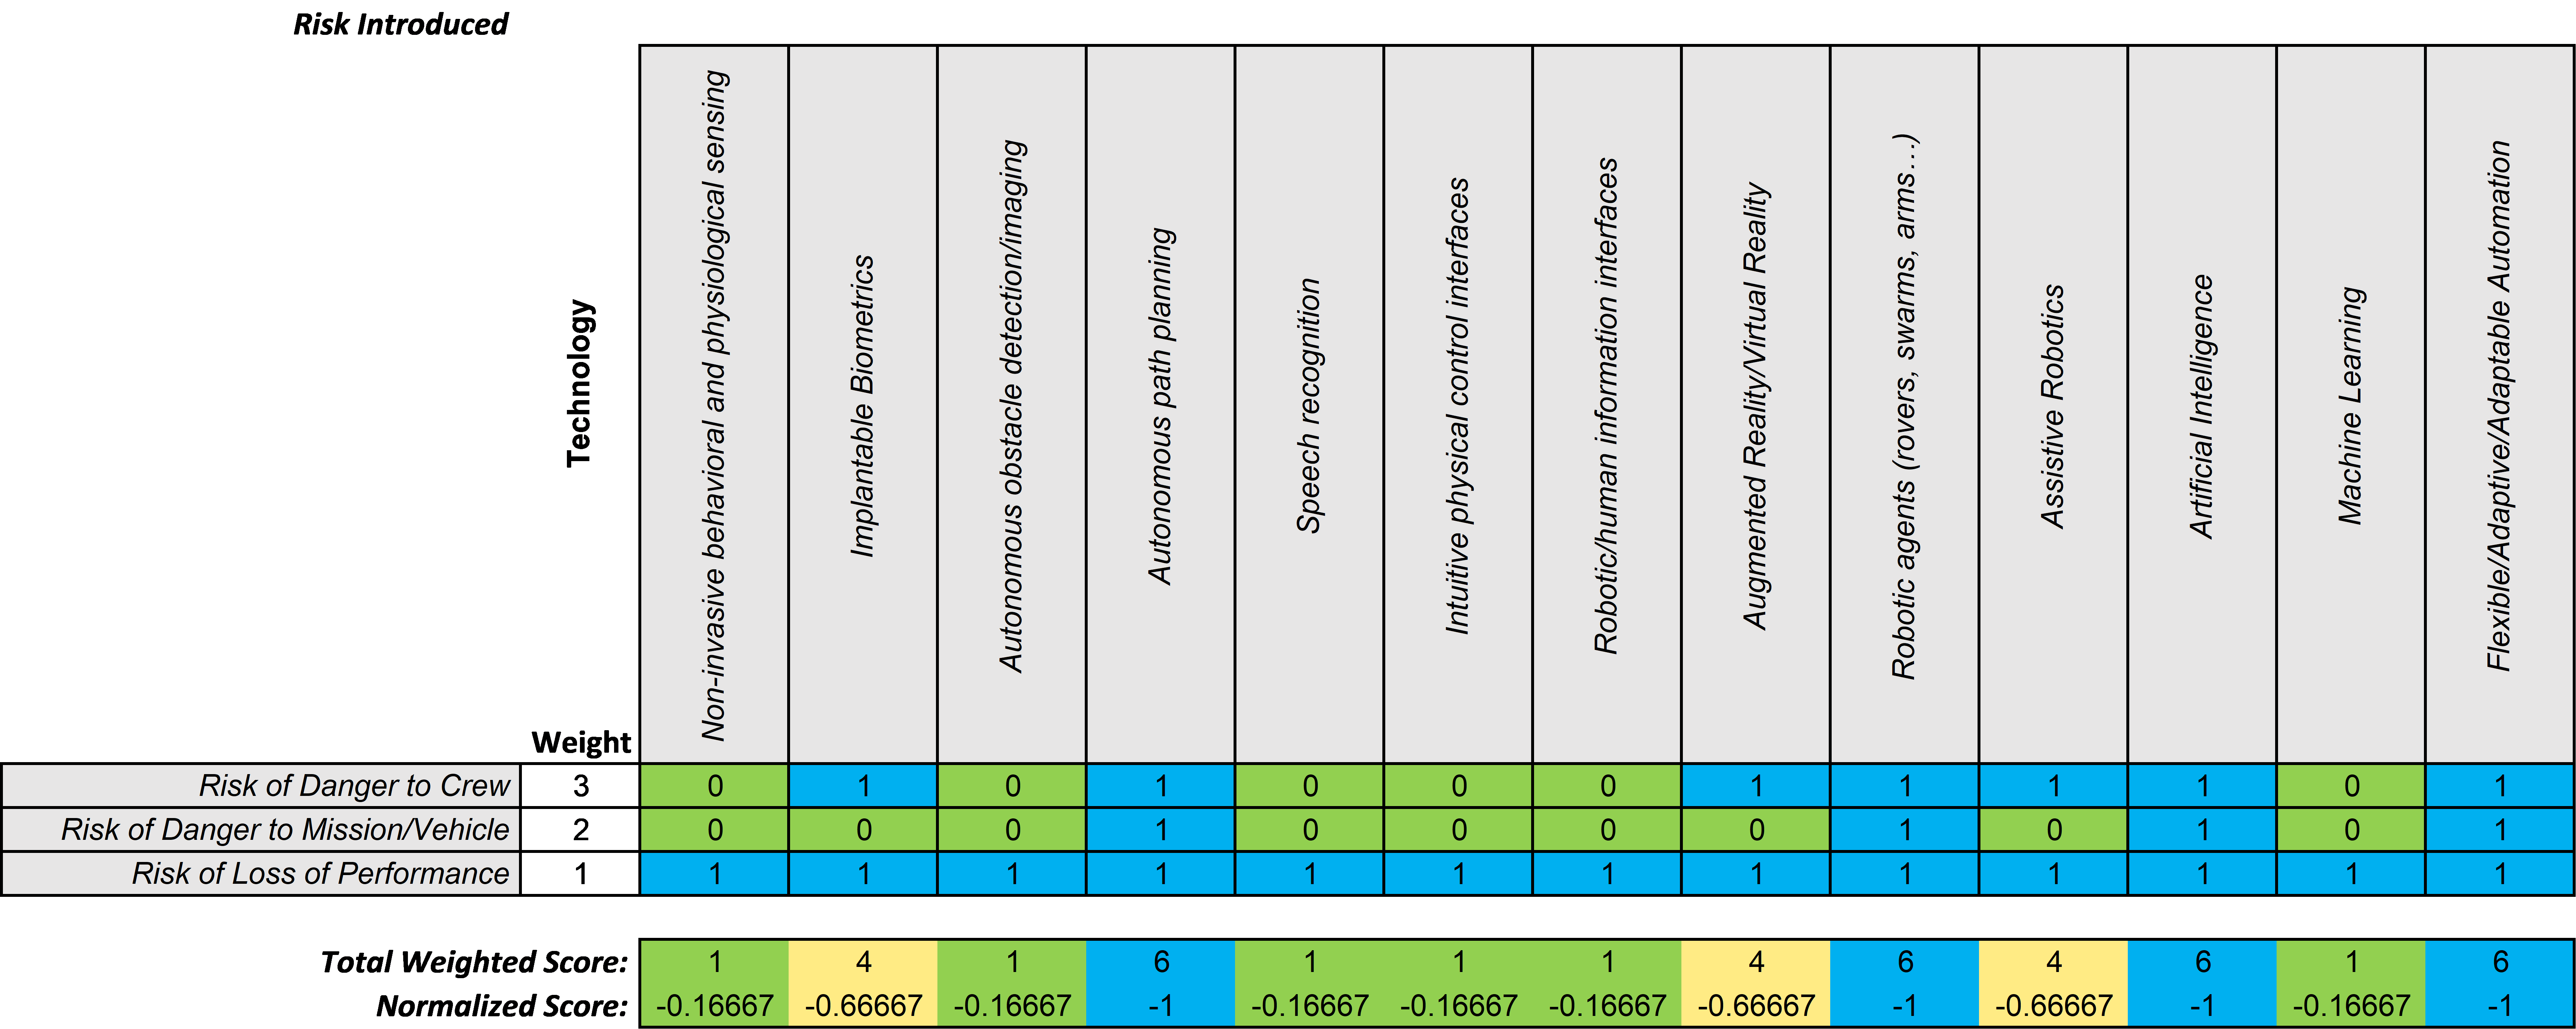
\includegraphics[width=0.8\linewidth]{figures/TradeStudy/figurea5.png}
        \caption[Technology to Risk Introduced factor-level trade table]{Technology to Risk Introduced factor-level trade table.}
        % \label{figure:}
    \end{center}
\end{figure}

\begin{figure}[b!]
    \begin{center}
        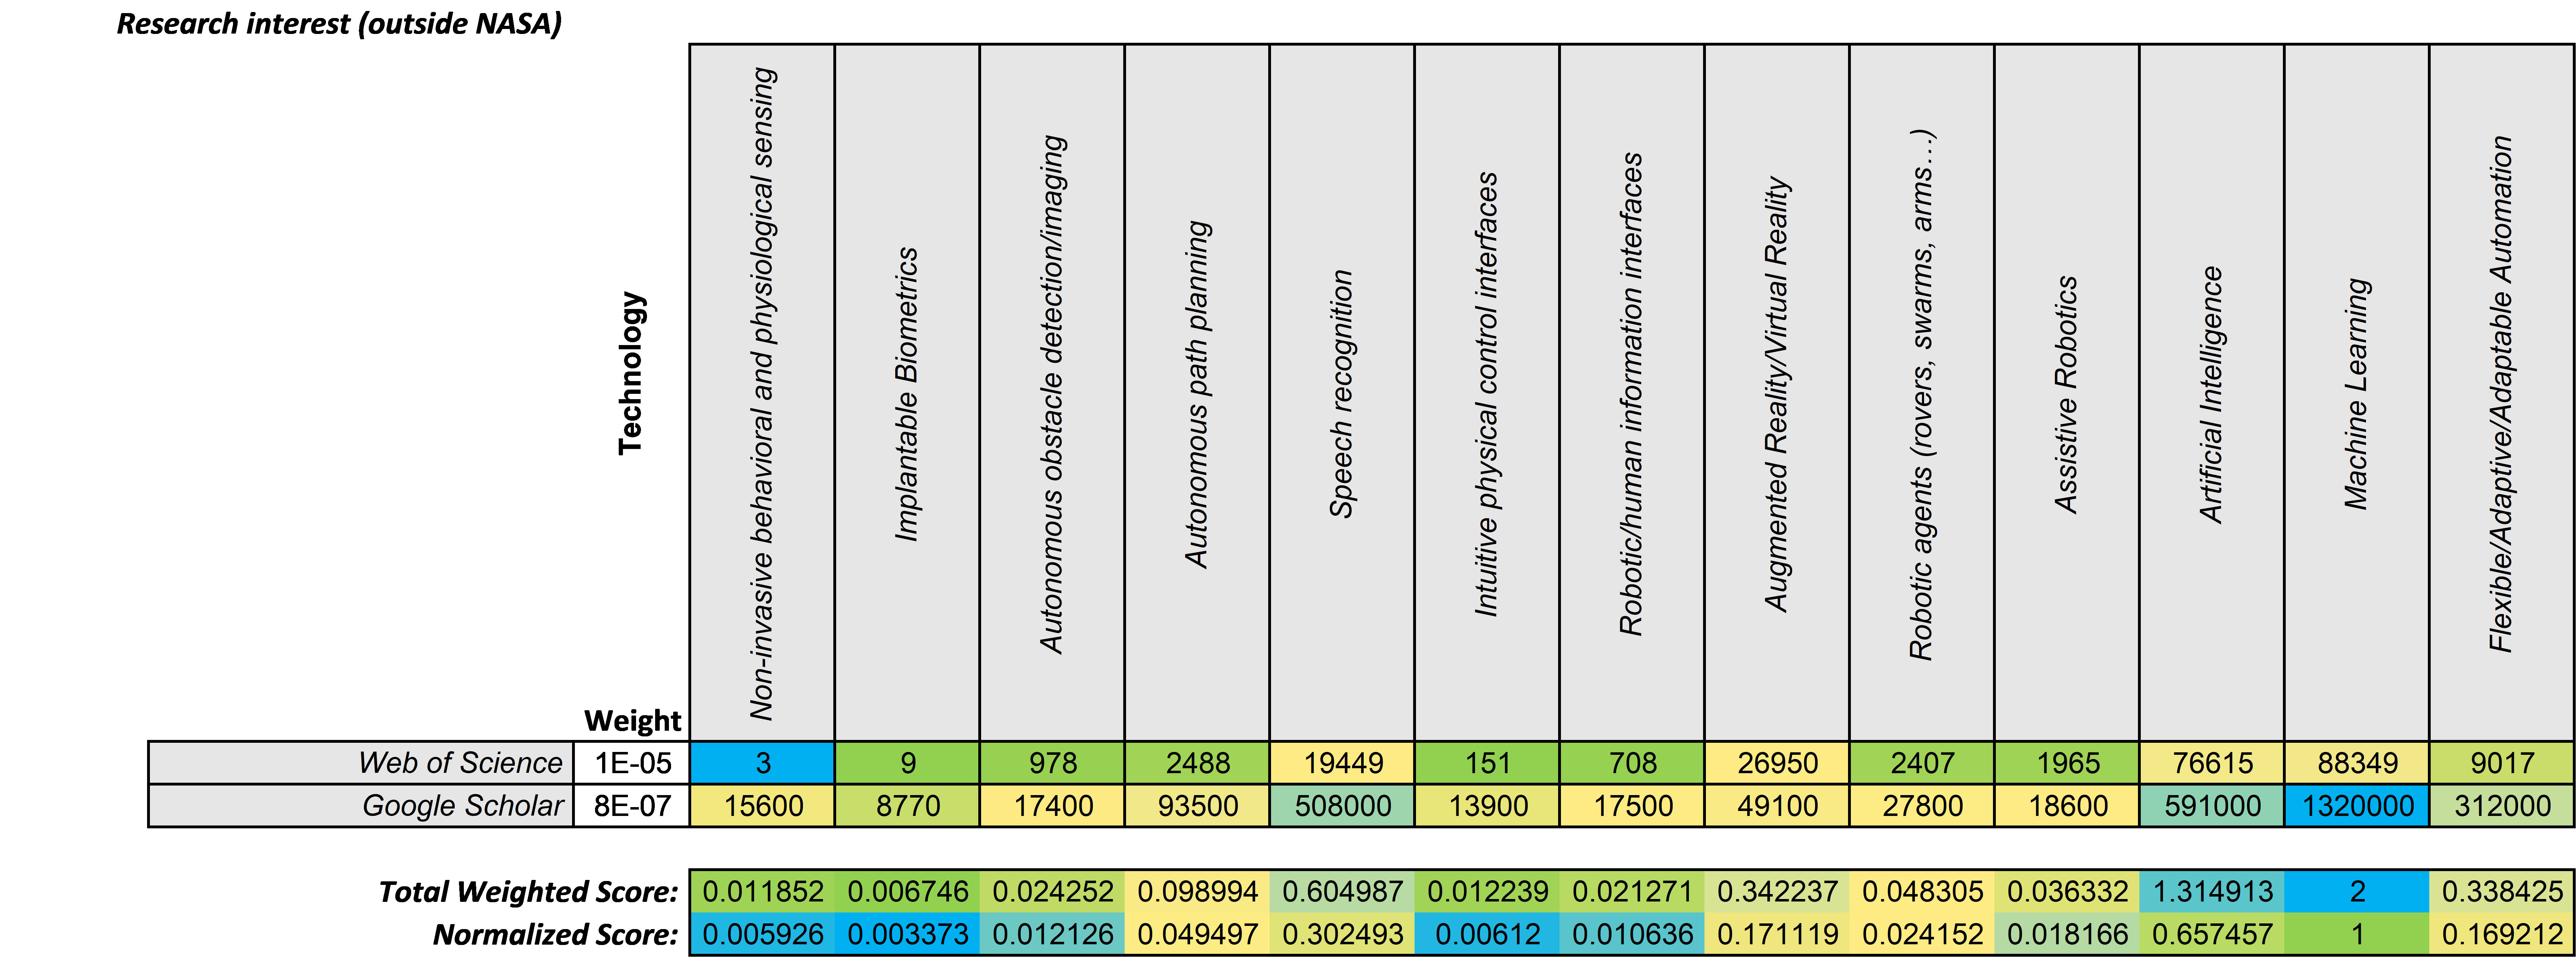
\includegraphics[width=0.8\linewidth]{figures/TradeStudy/figurea6.png}
        \caption[Technology to Research Interest (outside NASA) factor-level trade table]{Technology to Research Interest (outside NASA) factor-level trade table.}
        % \label{figure:}
    \end{center}
\end{figure}

\begin{figure}[b!]
    \begin{center}
        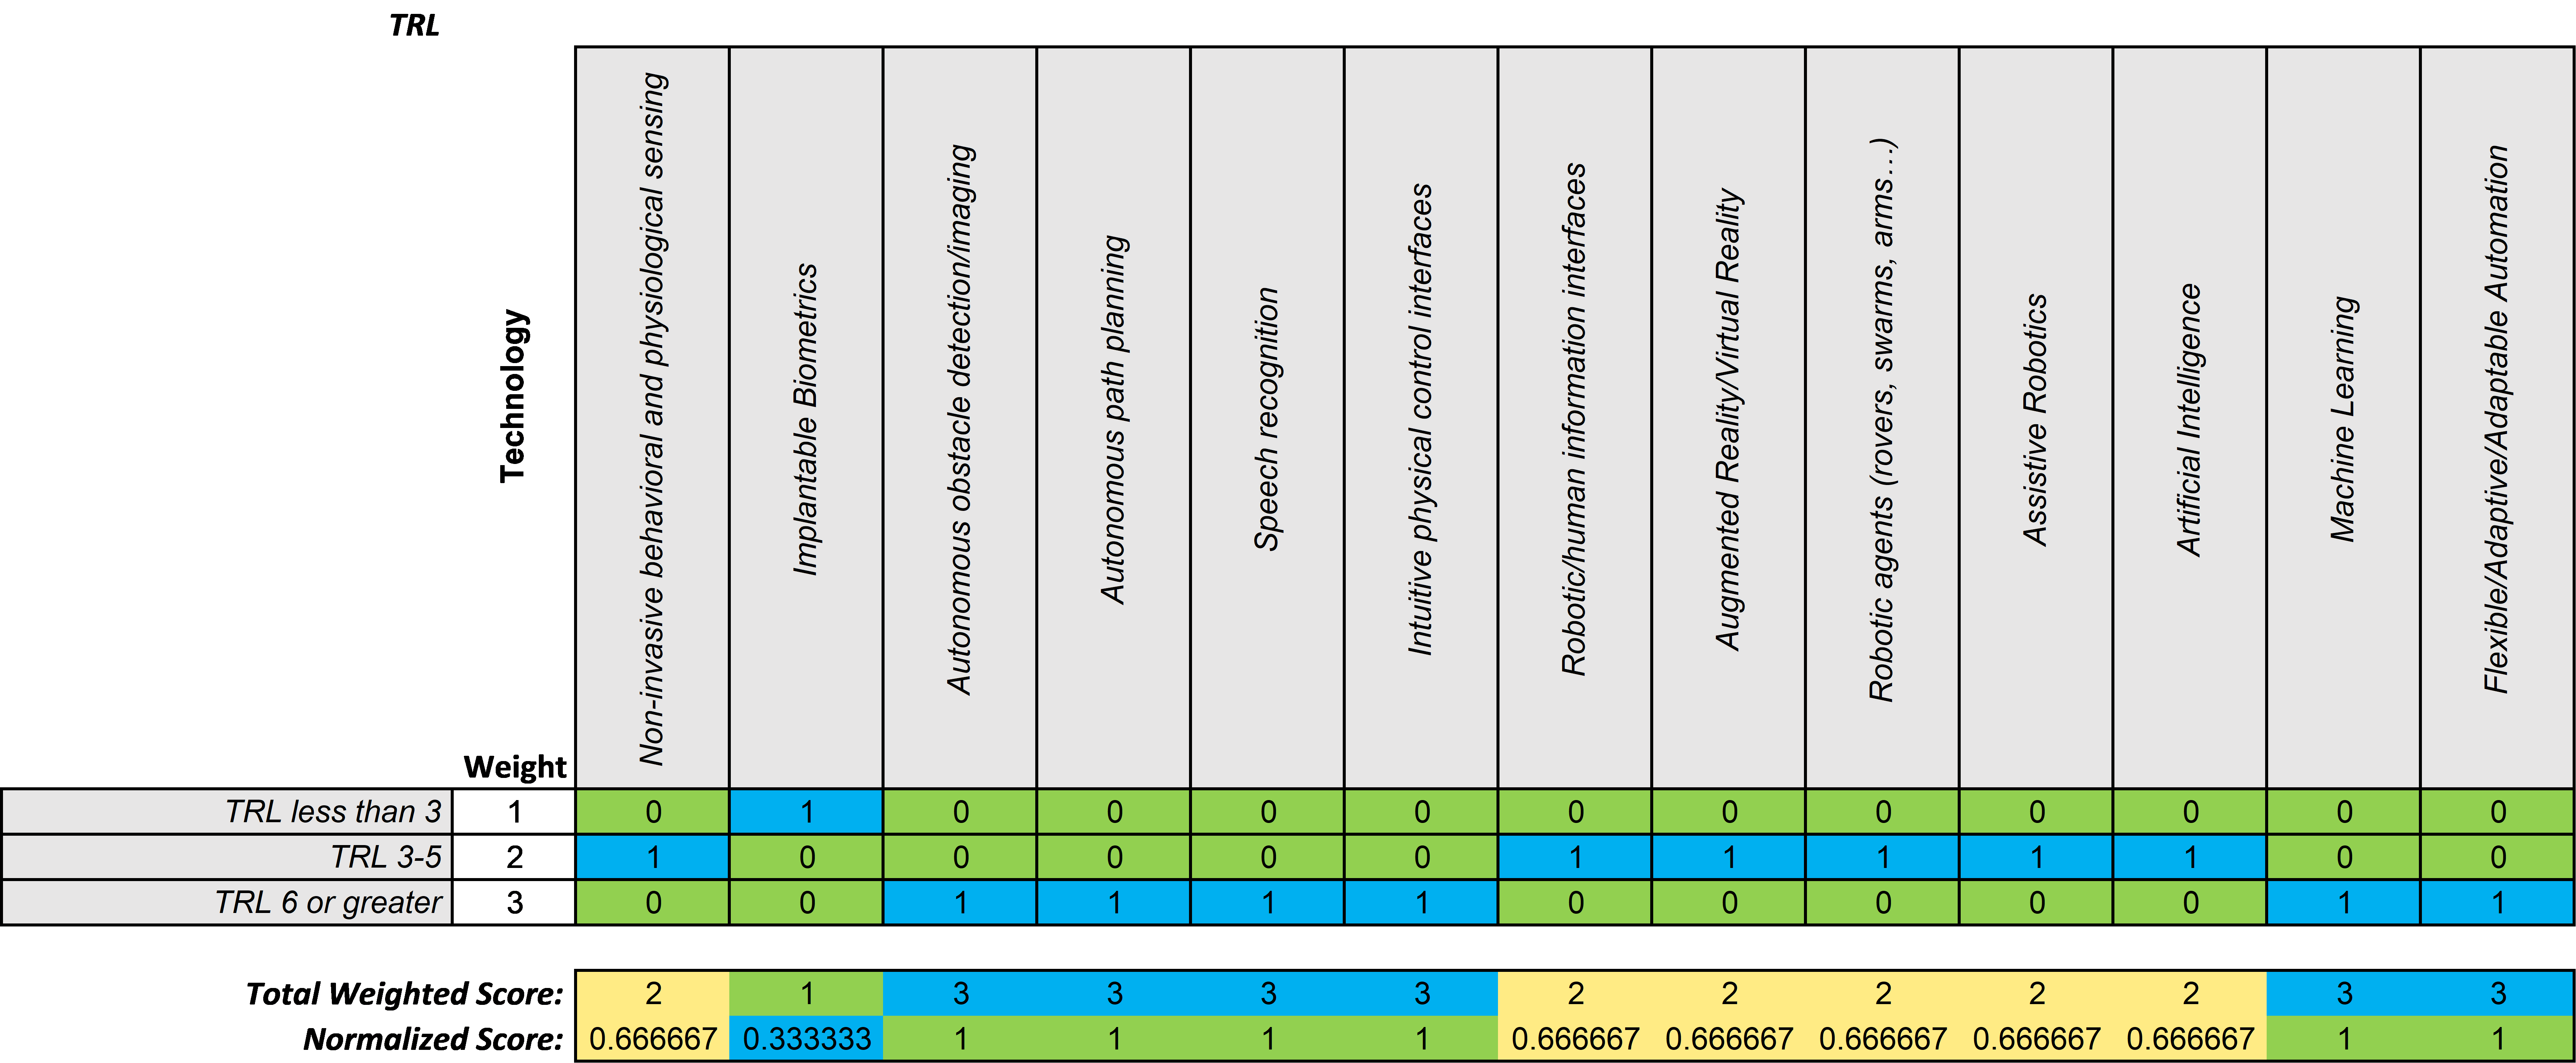
\includegraphics[width=0.8\linewidth]{figures/TradeStudy/figurea7.png}
        \caption[Technology to TRL factor-level trade table]{Technology to TRL factor-level trade table.}
        % \label{figure:}
    \end{center}
\end{figure}

\begin{figure}[b!]
    \begin{center}
        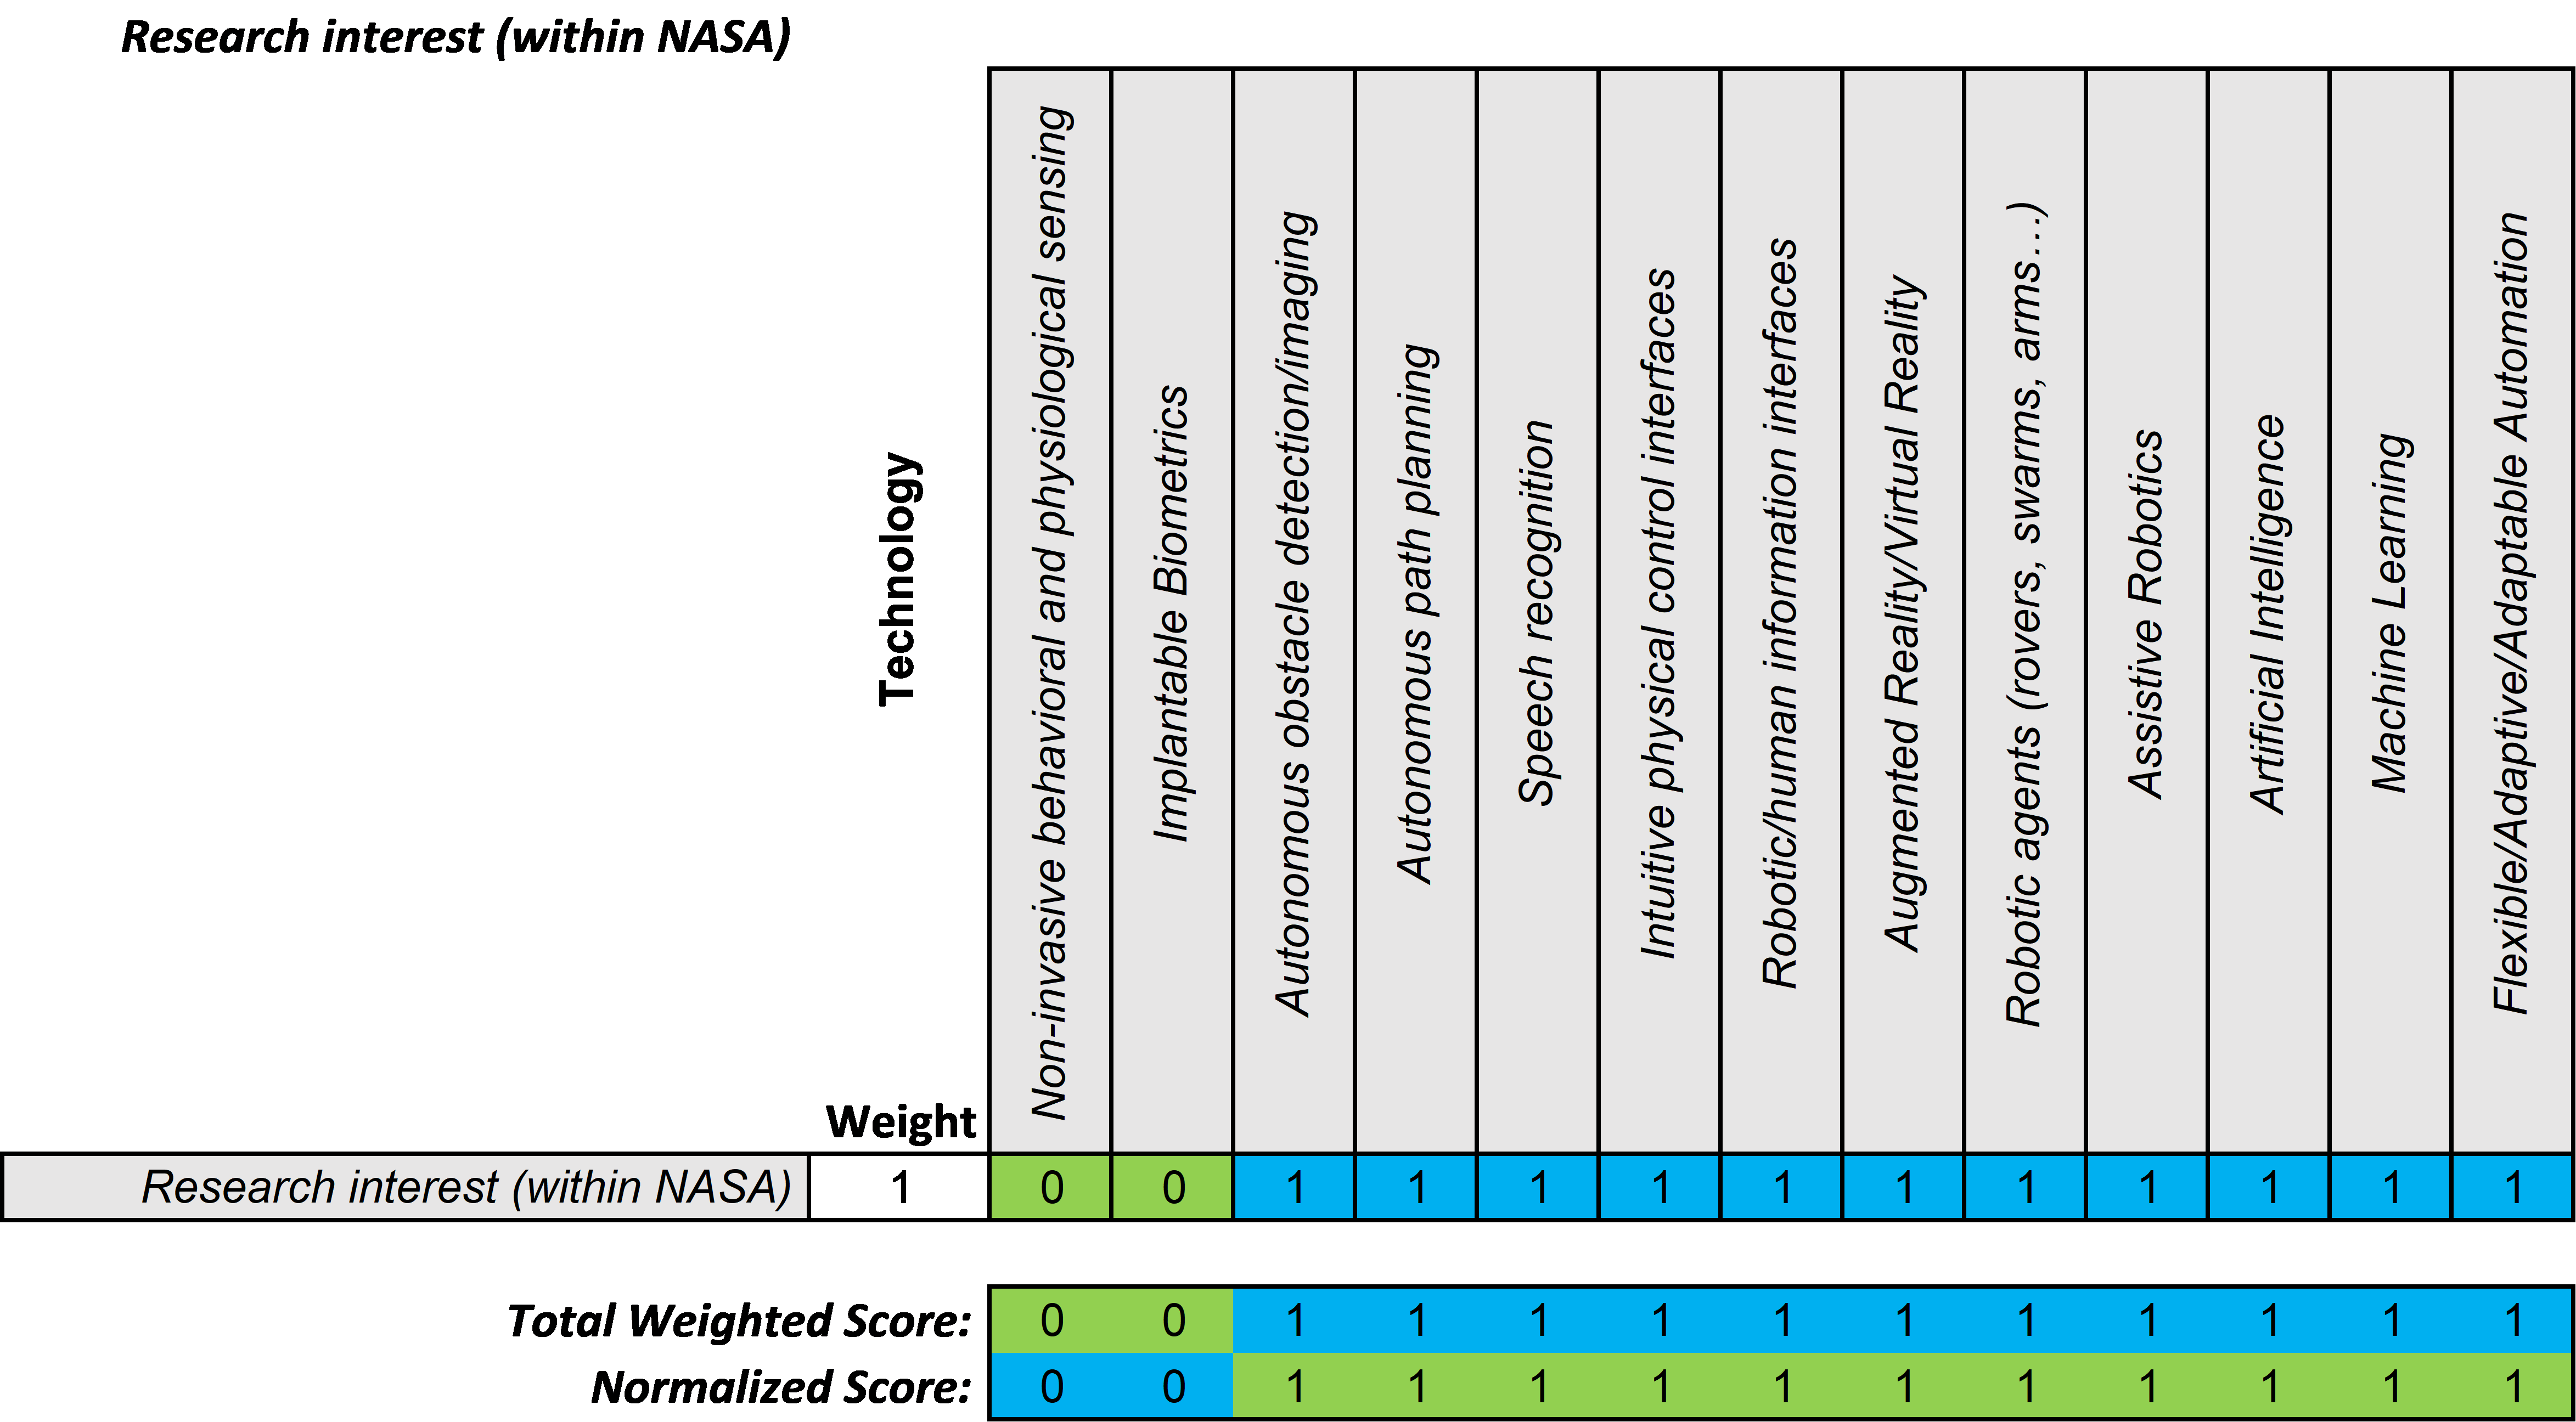
\includegraphics[width=0.8\linewidth]{figures/TradeStudy/figurea8.png}
        \caption[Technology to Research Interest (within NASA) factor-level trade table]{Technology to Research Interest (within NASA) factor-level trade table.}
        % \label{figure:}
    \end{center}
\end{figure}

% Appendix B: Subject Matter Expert Summary of Backgrounds
% The SMEs interviewed to gather background information on the HARI trade space all have extensive experience in either HAR integration research, human factors, or both, in their respective fields. Additionally, three SMEs have experience in related fields: one person in data analytics, and two others in psychology/neuroscience. The SMEs have a wide range of experience addressing different research applications, captured in Table B1.

% SME	Background	Expertise
% 		Space	Aviation	Military	Medical	Automotive	Locomotive	Robotics (general)
% 1	Industry		x	x
% 2	Industry		x	x
% 3	Academia	x	x			x	x	x
% 4	Industry,
% Former NASA	x	x		x
% 5	Military			x	x			x
% 6	Academia, Industry				x	x
% 7	Academia	x	x	x			x
% 8	Academia,
% Industry		x					x
% 9	Academia	x			x			x
% 10	Industry,
% Former NASA	x			x	x
% Table B1: Background and application area expertise of interviewed subject matter experts

\chapter{Aircraft Dynamics} \label{appendix:dynamics}

\section{Longitudinal Dynamics}
\begin{align*}
    \dot{\vec{x}}_{long} =
    \left[ \begin{array}{ *{5}{c} }
            X_u                     & X_w                     & X_q                                          & -g \cos \theta_0 & 0 \\
            Z_u                     & Z_w                     & Z_q + U_0                                    & -g \sin \theta_0 & 0 \\
            M_u + M_{\dot{w}} Z_{u} & M_w + M_{\dot{w}} Z_{w} & M_q + M_{\dot{w}} \left( Z_{q} + U_0 \right) & 0                & 0 \\
            0                       & 0                       & 1                                            & 0                & 0 \\
            0                       & -1                      & 0                                            & U_0              & 0 \\
        \end{array} \right]
    \left[ \begin{array}{ *{1}{c} }
            \Delta u      \\
            \Delta w      \\
            \Delta q      \\
            \Delta \theta \\
            \Delta z      \\
        \end{array} \right] & + \\
    \left[ \begin{array}{ *{5}{c} }
            X_{\delta_e}                            & X_{\delta_{th}}                               \\
            Z_{\delta_e}                            & Z_{\delta_{th}}                               \\
            M_{\delta_e} + M_{\dot{w}} Z_{\delta_e} & M_{\delta_{th}} + M_{\dot{w}} Z_{\delta_{th}} \\
            0                                       & 0                                             \\
            0                                       & 0                                             \\
        \end{array} \right]
    \left[ \begin{array}{ *{1}{c} }
            \Delta \delta_e    \\
            \Delta \delta_{th} \\
        \end{array} \right] &   \\
\end{align*}

\section{Lateral Dynamics}
\begin{align*}
    \dot{\vec{x}}_{lat} =
    \left[ \begin{array}{ *{5}{c} }
            Y_v  & Y_p  & Y_r - U_0     & g \cos \theta_0  & 0 \\
            L'_v & L'_p & L'_r          & -g \sin \theta_0 & 0 \\
            N'_v & N'_p & N'_r          & 0                & 0 \\
            0    & 1    & \tan \theta_0 & 0                & 0 \\
            0    & 0    & \sec \theta_0 & 0                & 0 \\
        \end{array} \right]
    \left[ \begin{array}{ *{1}{c} }
            \Delta v    \\
            \Delta p    \\
            \Delta r    \\
            \Delta \phi \\
            \Delta \psi \\
        \end{array} \right] & + \\
    \left[ \begin{array}{ *{5}{c} }
            Y_{\delta_{a}}  & Y_{\delta_{r}}  \\
            L'_{\delta_{a}} & L'_{\delta_{r}} \\
            N'_{\delta_{a}} & N'_{\delta_{r}} \\
            0               & 0               \\
            0               & 0               \\
        \end{array} \right]
    \left[ \begin{array}{ *{1}{c} }
            \Delta \delta_a \\
            \Delta \delta_r \\
        \end{array} \right] &   \\
\end{align*}
